\subsection{Setup}
This section demonstrates how a block based D-VTAGE value predictor improves the performance of core composition, with the round-robin fetch scheme.
The default fetching scheme is not explored as the previous section showed that even with a perfect value predictor performance does not improve.
This section introduces a new configuration for the core: Round Robin Fetch with D-VTAGE value prediction \nfvt{}.

The objective of this section is to demonstrate that a state of the art value predictor can be used to improve the performance of large core compositions, and to show the difference between a real predictor and the perfect predictor.
The D-VTAGE size configuration can be found in Table~\ref{tab:vtage-conf}.
The total memory budget for D-VTAGE was taken from Perais et al's original paper which introduced the predictor~\cite{}.

For this section, three features of the predictor are modified: the number of entries per block, whether a Forward Probabilistic Counter (FPC) is used, and the confidence required to use a prediction.
Modifying the required confidence and if the confidence is incremented using FPCs explores the trade-off beteween high coverage and low misprediction.
The original D-VTAGE paper used FPCs to increment the confidence, and only used predictions once the counter was set to 7.
This ensured that the predictor had an accuracy of over 99\%, but at the expense of a low coverage, 20\% on average.
Table~\ref{tab:vtage-params} shows the possible values that can be taken for the three parameters.



\begin{table}[t]
  \small
  \centering
 \begin{tabular} {| l | l | l |}
 \hline
	\#Base Ent. & \#Tagged & \#Spec Window\\ \hline
	256 & $6\times256$ & 64 \\ \hline
	\end{tabular}
  \caption{D-VTAGE table configuration.}\label{tab:vtage-conf}
  \vspace{1em}
\end{table}


\begin{table}[t]
\small
\centering
\begin{tabular}{p{5.2cm} p{1.8cm}}
\toprule
\textbf{Parameter} & \textbf{Values} \\ \midrule
\# of entries per block & 16 or 32\\
Forward Probabilistic Counters & On or Off \\
Confidence Value & 4 or 7 \\ \bottomrule
\end{tabular}
\caption{Configurable parameters for D-VTAGE}\label{tab:vtage-params}
\end{table}


\begin{table}[t]
\small
\centering
\begin{tabular}{p{5.2cm} p{1.8cm}}
\toprule
\textbf{Parameter} & \textbf{Values} \\ \midrule
\# of entries per block & 16 or 32\\
Forward Probabilistic Counters & On or Off \\
Confidence Value & 4 or 7 \\ \bottomrule
\end{tabular}
\caption{Configurable parameters for D-VTAGE}\label{tab:vtage-params}
\end{table}

\begin{table}[t]
  \small
  \centering
 \begin{tabular} {| l | l | l | l | l | l | }
 \hline
    & \cellcolor[gray]{0.7}Disparity & \cellcolor[gray]{0.7} Localization& \cellcolor[gray]{0.7} MSER& \cellcolor[gray]{0.7} Multi\_NCut& \cellcolor[gray]{0.7} Sift\\ \hline
 \vt   & 16  & 16 & 4  & 16& 16\\ \hline
 \nfvt   & 16  & 16 & 4  & 16& 16\\ \hline
	  & \cellcolor[gray]{0.7} Stitch & \cellcolor[gray]{0.7} SVM & \cellcolor[gray]{0.7} Text. Synth & \cellcolor[gray]{0.7} Tracking&\\ \hline
   \vt & 16  & 16 & 4  & 16 & \\ \hline
 \nfvt   & 16  & 16 & 4  & 16 &\\ \hline

	\end{tabular}
  \caption{Number of cores composed given a configuration.}\label{tab:conf_cores}
  \vspace{1em}
\end{table}


\subsection{Results}
\subsubsection{Performance}



\begin{figure}[t]
    \centering
    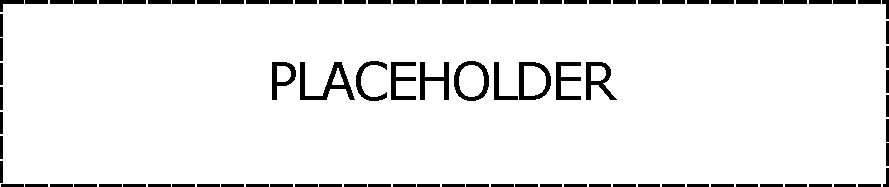
\includegraphics[width=1\textwidth]{chapter3/graphics/wip.pdf}
    \caption{Comparing the performance of the standard fetching scheme to the new fetching scheme, with and without perfect value prediction. Higher is better.}
    \label{fig:vtag_perf}
	\vspace{1em}
\end{figure}

\subsubsection{D-VTAGE Accuracy}
\begin{figure}[t]
    \centering
    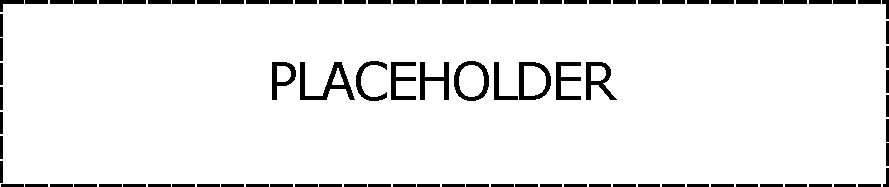
\includegraphics[width=1\textwidth]{chapter3/graphics/wip.pdf}
    \caption{Comparing the performance of the standard fetching scheme to the new fetching scheme, with and without perfect value prediction. Higher is better.}
    \label{fig:vtag_accuracy}
	\vspace{1em}
\end{figure}

\subsubsection{D-VTAGE Coverage}
\begin{figure}[t]
    \centering
    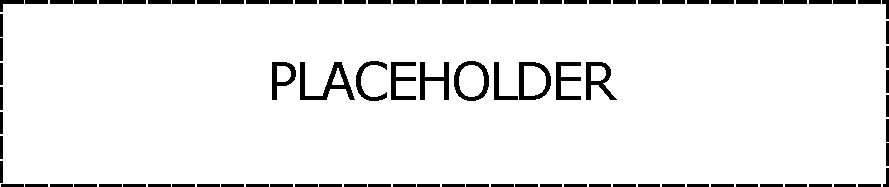
\includegraphics[width=1\textwidth]{chapter3/graphics/wip.pdf}
    \caption{Comparing the performance of the standard fetching scheme to the new fetching scheme, with and without perfect value prediction. Higher is better.}
    \label{fig:vtag_accuracy}
	\vspace{1em}
\end{figure}


\subsubsection{Changing counter requirements}
\begin{figure}[t]
    \centering
    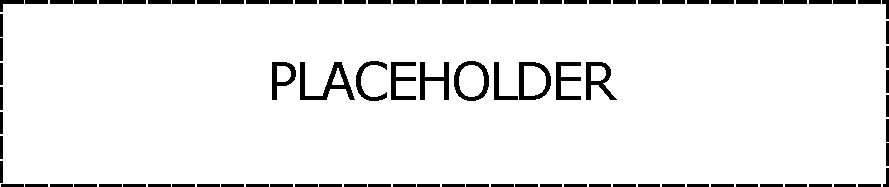
\includegraphics[width=1\textwidth]{chapter3/graphics/wip.pdf}
    \caption{Comparing the performance of the standard fetching scheme to the new fetching scheme, with and without perfect value prediction. Higher is better.}
    \label{fig:vtag_accuracy}
	\vspace{1em}
\end{figure}